\subsection{系统运行界面}

为了验证 FoodShield 系统的完整性和可展示性，本节从用户端、骑手端和管理员端三个角度展示系统运行界面。系统运行界面覆盖注册、登录、创建订单、订单通信、管理员登录、日志查看、Merkle 快照生成、完整性验证、条件溯源和三端摘要一致性等关键功能。

首先，用户端完成注册和登录后，可以创建订单并进入订单通信页面。订单创建成功后，系统生成随机订单号和订单 Token，用户端凭借订单号和 Token 加入对应通信房间。用户端页面展示订单状态、通信窗口和消息发送区域。

\begin{figure}[H]
    \centering
    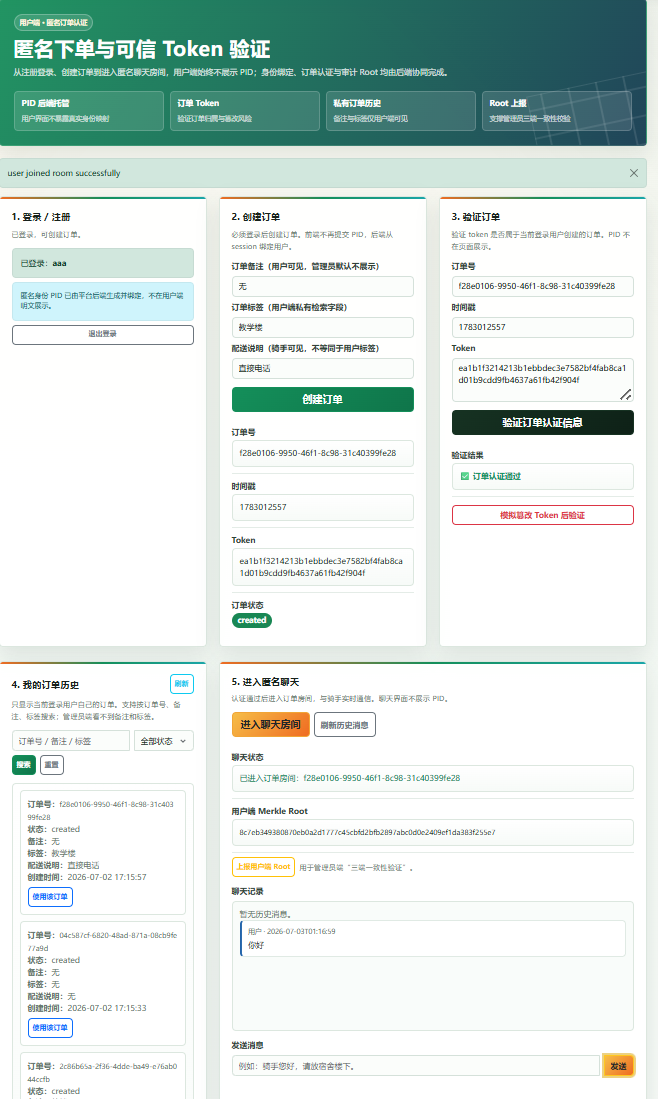
\includegraphics[width=0.95\textwidth]{content/chapter4/user_overview.png}
    \caption{用户端功能运行界面}
    \label{fig:user-overview}
\end{figure}

其次，骑手端可以查看订单并进入订单通信页面，与用户进行实时沟通。骑手端页面不展示用户真实身份和 PID，仅展示订单编号、订单状态和通信内容。该界面体现了系统的字段最小化展示原则。

\begin{figure}[H]
    \centering
    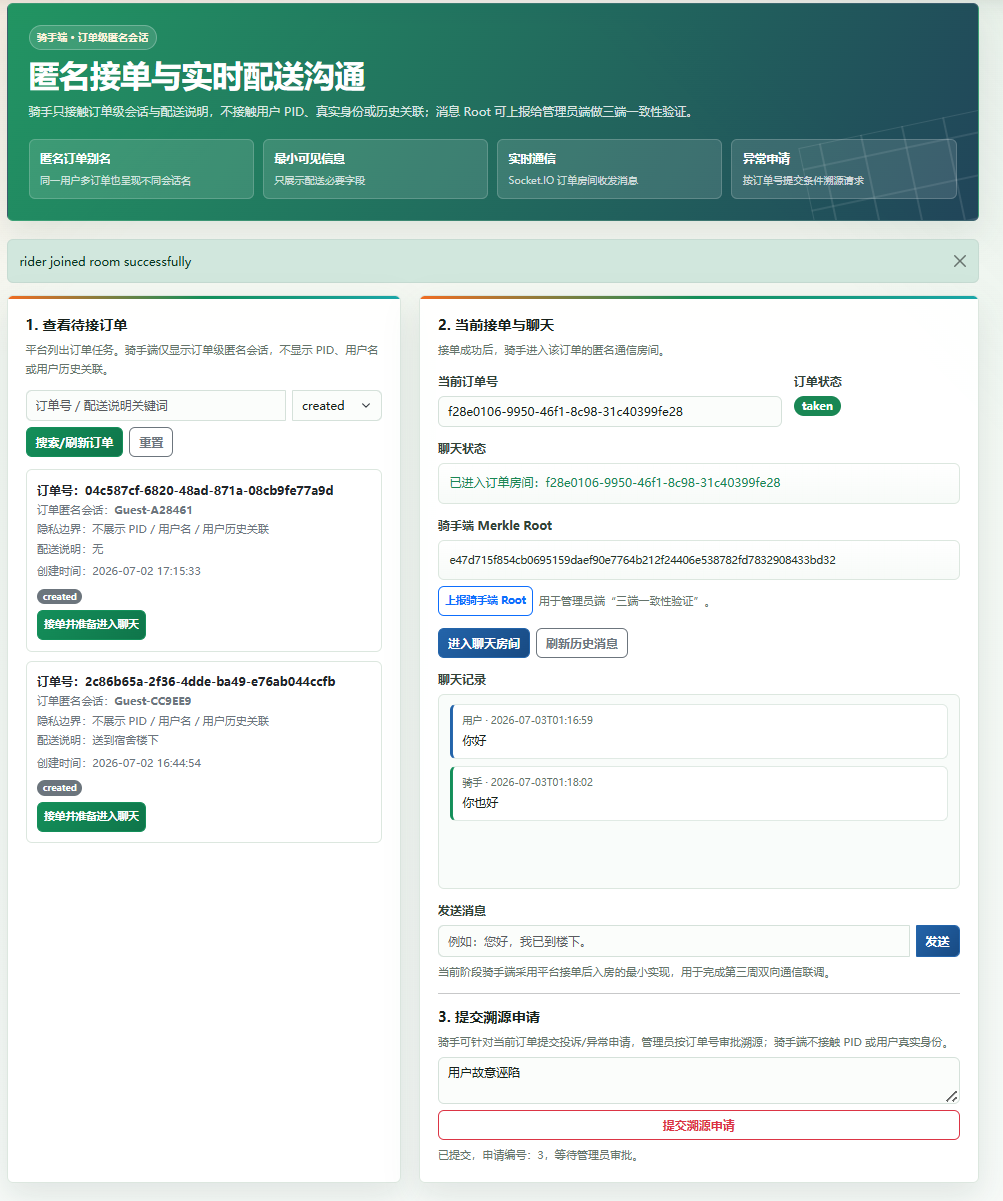
\includegraphics[width=0.95\textwidth]{content/chapter4/rider_overview.png}
    \caption{骑手端功能运行界面}
    \label{fig:rider-overview}
\end{figure}

再次，管理员端完成登录后，可以基于订单号查看订单审计摘要、消息哈希和 Merkle Root。管理员可以手动生成 Root 快照，也可以执行完整性验证。若日志未被篡改，系统返回验证通过；若消息记录被修改、删除、插入或重排，系统返回验证失败并记录审计日志。

\begin{figure}[H]
    \centering
    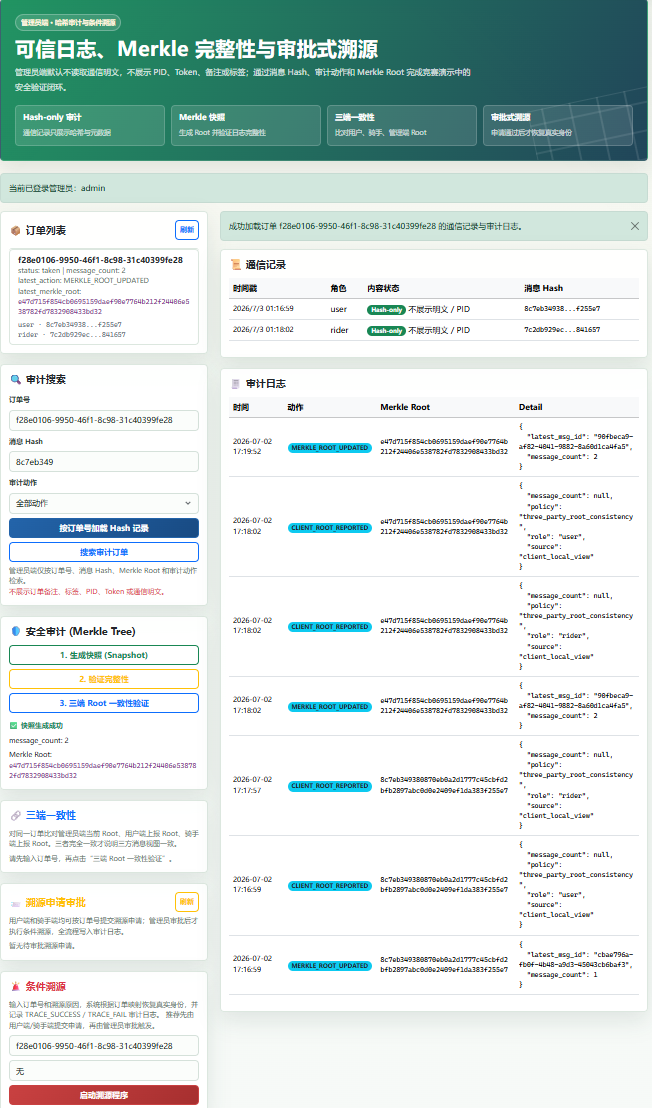
\includegraphics[width=0.85\textwidth]{content/chapter4/admin_audit_overview.png}
    \caption{管理员端日志审计界面}
    \label{fig:admin-audit-overview}
\end{figure}

最后，在异常场景下，用户端和骑手端均可提交溯源申请，管理员端根据订单号处理申请。系统先执行 Merkle 完整性验证，再进行关键词命中检测，最后在满足条件时返回溯源结果。该界面展示了 FoodShield 从匿名通信到可信审计再到条件溯源的完整闭环。

\begin{figure}[H]
    \centering
    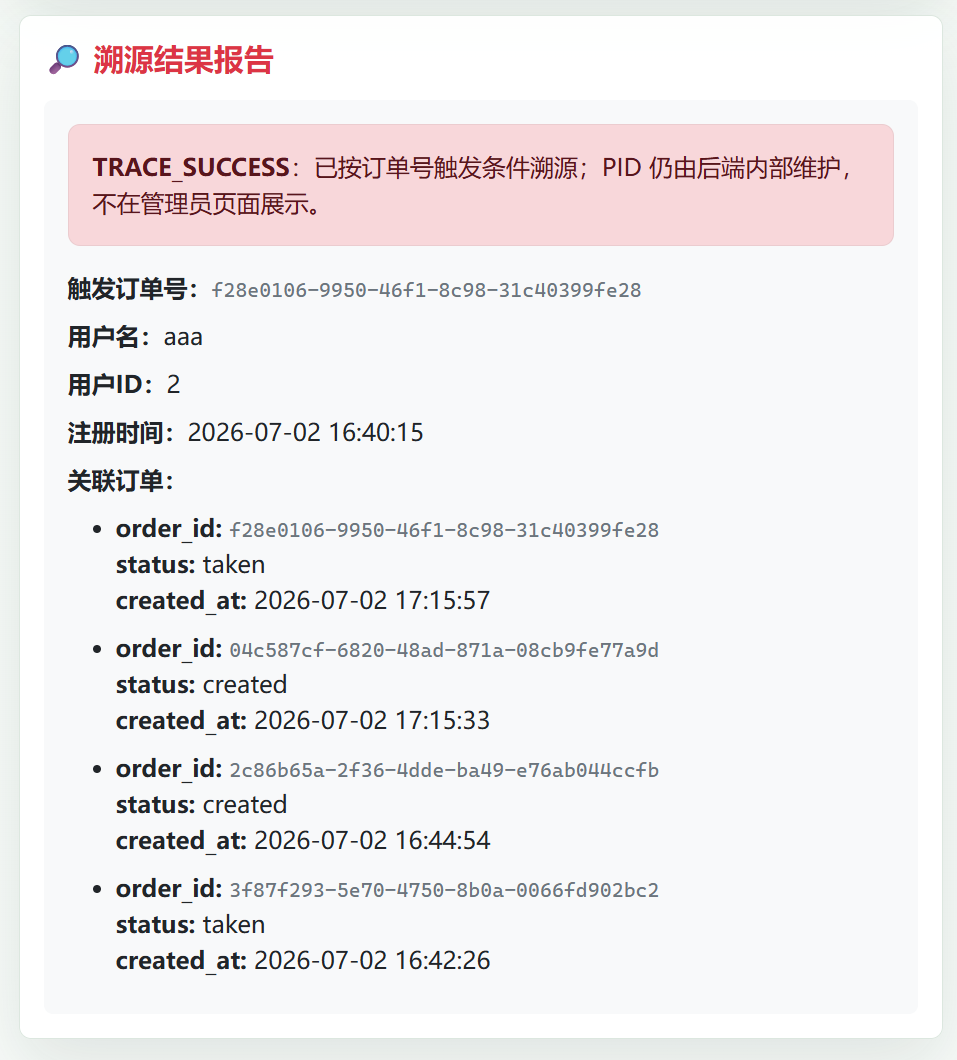
\includegraphics[width=0.95\textwidth]{content/chapter4/trace_overview.png}
    \caption{条件溯源功能运行界面}
    \label{fig:trace-overview}
\end{figure}

通过上述运行界面可以看出，FoodShield 已经实现了用户端、骑手端和管理员端的完整业务流程。系统不仅支持普通外卖订单通信，还在通信过程中集成了匿名身份、订单认证、消息加密、日志哈希、Merkle Root 快照、完整性验证和条件溯源等安全机制。相比普通聊天系统，FoodShield 的实现更强调隐私保护、权限边界和可信审计，能够较好地支撑外卖订单通信场景下的安全需求。
